% =====================================================================
%  CPE 334 - Lab 7 Submission : Software Maintenance Metrics & Release Readiness
%  Comprehensive Submission Report with Full Verifiable Evidence
% =====================================================================
\documentclass[10pt,a4paper]{article}
\usepackage[utf8]{inputenc}
\UseRawInputEncoding
\usepackage[T1]{fontenc}
\usepackage[a4paper,left=1.2cm,right=1.2cm,top=1.0cm,bottom=1.1cm]{geometry}
\usepackage{amsmath}
\usepackage{graphicx}
\usepackage{listings}
\usepackage{xcolor}
\usepackage{booktabs}
\usepackage{enumitem}
\usepackage{parskip}
\usepackage{amssymb}
\usepackage{array}
\usepackage{url}
\usepackage{hyperref}

\definecolor{tggreen}{HTML}{006B3C}
\definecolor{tgdark}{HTML}{1A365D}
\definecolor{codebg}{HTML}{F8FAFC}
\hypersetup{colorlinks=true, linkcolor=tggreen, urlcolor=tggreen}

\newcolumntype{L}[1]{>{\raggedright\arraybackslash}p{#1}}
\newcolumntype{C}[1]{>{\centering\arraybackslash}p{#1}}

\setlength{\extrarowheight}{2.0pt}
\setlength{\aboverulesep}{0.3ex}
\setlength{\belowrulesep}{0.4ex}

\newcommand{\partheader}[2]{%
  \vspace{4pt}%
  \noindent\textbf{\textcolor{tggreen}{\large #1}} \hfill \textbf{\small\textcolor{tgdark}{#2}}\par
  \vspace{2pt}\hrule height 0.8pt\vspace{4pt}%
}

\newcommand{\code}[1]{\texttt{\detokenize{#1}}}

\lstset{
  basicstyle=\ttfamily\tiny,
  breaklines=true,
  frame=single,
  backgroundcolor=\color{codebg},
  columns=fullflexible,
  captionpos=b,
  aboveskip=1.5pt,
  belowskip=1.5pt,
}

\setlength{\parskip}{2.0pt}
\setlength{\parindent}{0pt}

\begin{document}

% =====================================================================
% PAGE 1: Front Matter, Metadata, Evidence Index, Part A
% =====================================================================
\begin{center}
  \textcolor{tggreen}{\textbf{\large CPE 334 --- Lab 7 Submission: Software Maintenance Metrics \& Release Readiness}}\\[2pt]
  \normalsize Theme 5: Workflow and Approval System \quad$\vert$\quad Team Pluak Daeng (Section 1)\\[2pt]
  \small\textbf{Authors:} Siriwan Yindeepot (67070501075, @ssiriwan) \ \& \ Thanaboon Tikaew (67070501021, @thhanabun)\\[1pt]
  \footnotesize\url{https://github.com/ssiriwan/cpe334-approval-system} \quad$\vert$\quad Date: 27 November 2026
\end{center}
\vspace{-4pt}

\partheader{Part 0: Project Metadata and Evidence Index}{Overview}

\begin{center}
\footnotesize
\begin{tabular}{@{}L{3.2cm}L{14.0cm}@{}}
\toprule
\textbf{Attribute} & \textbf{Deployment / Repository Value} \\
\midrule
Application \& Theme & Theme 5 Workflow \& Approval System --- \url{https://sd3cdaba1-4d7hbszvwq-as.a.run.app} \\
Accepted Sprint 1 Baseline & Tag \code{v0.1.0-sprint1} $\vert$ Commit \code{f35ad24ede42ed5522b20a68179473bf286744f3} (Old behavior baseline) \\
Pre-Change Commit & Commit \code{e695264} (\code{main} branch at Lab 7 start; includes Lab 5 CI/CD and Lab 6 UAT fixes) \\
Submitted Release Commit & Commit \code{a5b963650bcbdd3178609c551634638e927a08f7} (Release PR \#64 merged to \code{main}) \\
Cloud Run Live Revision & \code{sd3cdaba1-00012-skm} (100\% traffic, serving release commit \code{a5b9636}) \\
Health Check Endpoint & \code{GET /api/health} $\to$ \code{{"status":"ok","commit":"a5b9636...","timestamp":"2026-11-27T07:05:38Z"}} \\
\bottomrule
\end{tabular}
\end{center}
\vspace{1pt}

\begin{center}
\footnotesize
\begin{tabular}{@{}C{1.8cm}L{5.8cm}C{1.6cm}L{8.0cm}@{}}
\toprule
\textbf{Section} & \textbf{Topic / Milestone} & \textbf{Page} & \textbf{Primary Evidence Identifiers} \\
\midrule
\textbf{Part A} & Approved Change Request \& Contract v1.1 (25 pts) & Page 1--2 & CR-04, Trace Table, SRS BR-05 v1.1, STS TEST-01a..01f, PR \#61 \\
\textbf{Part B} & TDD Implementation \& Regression Suite (50 pts) & Page 2--3 & RED \code{2b56a7b}, GREEN \code{fede788}, PR \#63, 43/43 tests pass, diff \\
\textbf{Part C} & 5 Metrics, Interpretation \& Readiness Checklist (25 pts) & Page 4 & Issues, PRs, Tests, Defects, CI runs, 82-word risk interpretation \\
\textbf{Part D} & Retrospective, Live Cloud Run Evidence \& Appendix & Page 5--6 & Ready verdict, Retro, Live logs \code{EV-L7-DEPLOY-01}, 2 Screenshots \\
\bottomrule
\end{tabular}
\end{center}
\vspace{1pt}

\partheader{Part A: Approved Change Request \& Contract Revision v1.1}{25 Points}

\textbf{1. Change Request Identification (CR-04):}
\begin{itemize}[leftmargin=*,itemsep=1pt,topsep=1pt]
  \item \textbf{Target System Requirement:} FR-02 (Request Creation), FR-06 (Reviewer Queue) and \textbf{BR-05} (Reviewer Assignment).
  \item \textbf{Location in Codebase:} \code{server/src/services/request.service.ts} (\code{resolveAssignedReviewerId}, \code{createRequest}).
  \item \textbf{Reason for Change:} Sprint 1 used deterministic category-only assignment, ignoring transaction magnitude and submission time. CR-04 escalates high-value ($> 5,000.00$ THB) or after-hours ($< 08:00$ or $\ge 18:00$ Asia/Bangkok) requests to \code{manager.hybrid@cpe334.local} so experienced approvers handle higher operational risk, while preserving strict self-approval and access controls.
\end{itemize}

\textbf{2. Exact Old Rule vs. New Rule Specification:}
\begin{center}
\footnotesize
\begin{tabular}{@{}L{2.8cm}L{6.8cm}L{7.4cm}@{}}
\toprule
\textbf{Dimension} & \textbf{Old Rule (Accepted Sprint 1 Baseline)} & \textbf{New Rule (Approved Maintenance CR-04)} \\
\midrule
Normal Requests & EQUIPMENT/TRAVEL $\to$ \code{t.reviewer}; SOFTWARE/SUPPLIES $\to$ \code{manager.hybrid} & \textbf{Preserved unchanged} for amount $\le 5,000.00$ THB within 08:00--17:59 ICT. \\
High-Value Requests & Category-only mapping regardless of amount & Amount $> 5,000.00$ THB $\to$ \textbf{Escalate to \code{manager.hybrid}}. \\
Time Boundary & No time-of-day rule & Submission $< 08:00$ or $\ge 18:00$ Asia/Bangkok $\to$ \textbf{Escalate to \code{manager.hybrid}}. \\
Self-Approval Guard & Alternate reviewer if requester is primary & \textbf{Preserved unchanged} (BR-01): Escalated reviewer who is requester falls back to \code{t.reviewer}. \\
Client-Supplied Field & Ignored or stripped & Explicitly rejected with \code{400 VALIDATION_ERROR}; schema stays \code{.strict()}. \\
Database Schema & Nullable \code{assignedReviewerId} column & \textbf{Zero schema changes, zero migrations}; existing column reused. \\
\bottomrule
\end{tabular}
\end{center}
\vspace{1pt}

\textbf{3. Scope Boundaries and Invariant Safety:}
\begin{itemize}[leftmargin=*,itemsep=1pt,topsep=1pt]
  \item \textbf{Exact Boundaries:} Amount $5,000.00$ THB at 10:00 ICT $\to$ \code{t.reviewer} (normal); $5,000.01$ THB at 10:00 ICT $\to$ \code{manager.hybrid} (escalated). Submission at 07:59 ICT $\to$ \code{manager.hybrid} (out-of-hours); 08:00 ICT $\to$ \code{t.reviewer} (in-hours); 17:59 ICT $\to$ \code{t.reviewer}; 18:00 ICT $\to$ \code{manager.hybrid}.
  \item \textbf{Negative / Invalid Cases:} Negative/zero amounts, invalid categories, descriptions $<10$ chars continue to be rejected with \code{400 VALIDATION_ERROR} (AC-02). Unauthenticated requests return \code{401 AUTH_REQUIRED}. Cross-user access returns \code{403 ACCESS_DENIED}.
\end{itemize}

\clearpage
% =====================================================================
% PAGE 2: Part A (Cont.) Impact Analysis & Part B (Implementation)
% =====================================================================
\partheader{Part A (Cont.): Impact Analysis \& Contract Revision v1.1}{Specification Trace}

\textbf{4. Impact Analysis Trace Table:}
\begin{center}
\footnotesize
\begin{tabular}{@{}L{2.2cm}L{2.8cm}L{2.2cm}L{4.0cm}L{5.4cm}@{}}
\toprule
\textbf{Requirement} & \textbf{SRS / SDS Section} & \textbf{AC / STS ID} & \textbf{Code Module} & \textbf{Impact \& Rationale} \\
\midrule
FR-02, BR-05 & \path{docs/srs.md} \S BR-05 & AC-01, TEST-01 & \code{server/src/.../request.service.ts} & \textbf{Direct Change:} Reviewer assignment logic altered based on amount and submission time boundaries. \\
FR-06 Review Queue & \path{docs/srs.md} \S FR-06 & AC-05, TEST-05 & \code{server/src/.../review.service.ts} & \textbf{Indirect Only:} Reads \code{assignedReviewerId}; no code change. Regression confirms pending queue separation. \\
BR-01 Self-Approval & \path{docs/srs.md} \S BR-01 & AC-07, TEST-08 & \code{server/src/.../review.service.ts} & \textbf{Must Remain Unchanged:} Enforced before assignment; fallback must never assign requester as reviewer. \\
BR-06 History Log & \path{docs/srs.md} \S BR-06 & AC-11, TEST-13 & \code{server/src/.../request.service.ts} & \textbf{Unchanged:} Reuses single \code{SUBMITTED} history row created within the existing database transaction. \\
Database Schema & \path{prisma/schema.prisma} & NFR-03 & Database Table \code{ApprovalRequest} & \textbf{N/A (Zero Change):} Reuses existing column \code{assignedReviewerId}; zero migrations, zero historical data drift. \\
\bottomrule
\end{tabular}
\end{center}
\vspace{1pt}

\textbf{5. Revised Contract Specification Excerpts (SRS \& Feature SDS v1.1):}
\begin{itemize}[leftmargin=*,itemsep=1pt,topsep=1pt]
  \item \textbf{SRS BR-05 v1.1 (Reviewer Assignment):} Every request must have an \code{assignedReviewerId}. For requests created after release v1.1: (a) amounts $\le 5,000.00$ THB submitted within 08:00--17:59 Asia/Bangkok retain category mapping; (b) amounts $> 5,000.00$ THB or submissions outside 08:00--17:59 Asia/Bangkok escalate to \code{manager.hybrid@cpe334.local}; (c) if the selected reviewer is the requester, fallback to alternate reviewer (\code{t.reviewer@cpe334.local}); (d) client-supplied assignment field rejected with \code{400 VALIDATION_ERROR}.
  \item \textbf{Feature SDS F-02 v1.1:} \code{POST /api/requests} executes \code{resolveAssignedReviewerId(tx, category, requesterId, amount, now)} inside transaction. Time is evaluated in Asia/Bangkok (UTC+7) using \code{Intl.DateTimeFormat}.
  \item \textbf{New Software Test Specifications (STS):} \code{TEST-01a} (EQUIPMENT $5000.00$ in-hours $\to$ \code{t.reviewer}); \code{TEST-01b} (EQUIPMENT $5000.01$ in-hours $\to$ \code{manager.hybrid}); \code{TEST-01c} (Time boundary 07:59 $\to$ manager, 08:00 $\to$ \code{t.reviewer}); \code{TEST-01d} (Time boundary 17:59 $\to$ \code{t.reviewer}, 18:00 $\to$ manager); \code{TEST-01e} (Client-supplied reviewer rejected 400); \code{TEST-01f} (Manager requester self-approval fallback $\to$ \code{t.reviewer}).
\end{itemize}

\textbf{6. Review and Approval Record \& Process Disclosure:}
\begin{itemize}[leftmargin=*,itemsep=1pt,topsep=1pt]
  \item \textbf{Instructor/TA Pre-Approval:} Course staff waived synchronous pre-approval for Lab 7; recorded honestly as \textbf{NOT AVAILABLE} in \path{docs/labs/lab-07/change-request.md}.
  \item \textbf{Teammate Contract Review:} Documented in PR \#61 (authored by Thanaboon, reviewed and merged by Siriwan into \code{lab7-staging} at commit \code{1ecda5b}). Substantive peer review of implementation vs contract was completed in PR \#63 (authored by Siriwan, reviewed and merged by Thanaboon). Sequence deviation is honestly disclosed in Part D.
\end{itemize}

\partheader{Part B: TDD RED/GREEN Implementation \& Verification}{50 Points}

\textbf{1. Test-Driven Development (TDD) Workflow:}
We strictly adhered to the Test-First RED $\to$ GREEN sequence. All 6 new boundary/security tests (\code{TEST-01a..01f}) were committed to \code{server/tests/requests.test.ts} before modifying implementation code.

\begin{center}
\footnotesize
\begin{tabular}{@{}L{1.8cm}C{1.8cm}L{6.6cm}C{2.0cm}L{4.8cm}@{}}
\toprule
\textbf{Phase} & \textbf{Commit} & \textbf{Verification Action} & \textbf{Test Outcome} & \textbf{Primary Evidence} \\
\midrule
\textbf{RED Phase} & \code{2b56a7b} & Added 6 boundary tests to test file. Verified against pre-change implementation (\code{1ecda5b}). & \textbf{3 Failed, 3 Passed} (Expected genuine RED) & \path{evidence/red-test-output.txt} (\code{EV-L7-RED-01}) \\
\textbf{GREEN Phase} & \code{fede788} & Implemented \code{resolveAssignedReviewerId} with Bangkok hour and amount escalation. & \textbf{43/43 Passed} (100\% Pass Rate) & \path{evidence/green-test-output.txt} (\code{EV-L7-GREEN-01}) \\
\bottomrule
\end{tabular}
\end{center}
\vspace{1pt}

\textbf{2. Genuine RED Failure Analysis (\code{EV-L7-RED-01}):}
Running Vitest on commit \code{2b56a7b} produced exactly 3 genuine failures and 3 passing invariant guards:
\begin{itemize}[leftmargin=*,itemsep=1pt,topsep=1pt]
  \item \textbf{\code{TEST-01b} (FAIL):} Amount $>5000.00$ THB expected \code{manager.hybrid}, received \code{t.reviewer} (baseline lacked amount escalation).
  \item \textbf{\code{TEST-01c} (FAIL):} 07:59 ICT expected \code{manager.hybrid}, received \code{t.reviewer} (baseline lacked morning boundary).
  \item \textbf{\code{TEST-01d} (FAIL):} 18:00 ICT expected \code{manager.hybrid}, received \code{t.reviewer} (baseline lacked evening boundary).
  \item \textbf{\code{TEST-01a, 01e, 01f} (PASS):} Preserved invariant guards (normal category mapping, strict schema rejection, self-approval fallback).
\end{itemize}

\clearpage
% =====================================================================
% PAGE 3: Part B (Cont.) Code Diff & Regression Suite
% =====================================================================
\partheader{Part B (Cont.): Implementation Code Diff \& Regression Suite}{Bounded Modification}

\textbf{3. Exact Implementation Code Diff (\code{server/src/services/request.service.ts}):}
\begin{lstlisting}[language=Java]
function getBangkokHour(date: Date): number {
  const formatter = new Intl.DateTimeFormat('en-US', { timeZone: 'Asia/Bangkok', hour: 'numeric', hour12: false });
  return Number.parseInt(formatter.format(date), 10);
}

export async function resolveAssignedReviewerId(
  tx: Prisma.TransactionClient, category: RequestCategory, requesterId: string, amount: number, now: Date = new Date()
): Promise<string> {
  const primaryEmail = CATEGORY_PRIMARY_REVIEWER[category];
  const fallbackEmail = CATEGORY_FALLBACK_REVIEWER[category];

  // Evaluate CR-04 escalation boundary (>5000 THB or out-of-hours <08:00 or >=18:00 ICT)
  const bangkokHour = getBangkokHour(now);
  const isOutOfHours = bangkokHour < 8 || bangkokHour >= 18;
  const isHighValue = amount > 5000.00;
  const shouldEscalate = isHighValue || isOutOfHours;
  const targetEmail = shouldEscalate ? 'manager.hybrid@cpe334.local' : primaryEmail;

  const candidate = await tx.user.findUnique({ where: { email: targetEmail }, select: { id: true, role: true } });
  if (candidate && candidate.id !== requesterId && (candidate.role === 'REVIEWER' || candidate.role === 'ADMIN')) {
    return candidate.id;
  }

  // Fallback to alternate reviewer to preserve BR-01 self-approval invariant
  const fallback = await tx.user.findUnique({
    where: { email: shouldEscalate ? fallbackEmail : 't.reviewer@cpe334.local' }, select: { id: true, role: true }
  });
  if (fallback && fallback.id !== requesterId && (fallback.role === 'REVIEWER' || fallback.role === 'ADMIN')) {
    return fallback.id;
  }
}
\end{lstlisting}
\vspace{-2pt}

\textbf{4. Full Regression Suite Results across Stack (\code{EV-L7-GREEN-01}):}
Full test suite executed against release commit \code{a5b9636}. All 7 suites and 43 tests passed with 0 regressions.
\begin{center}
\footnotesize
\begin{tabular}{@{}L{5.0cm}C{1.4cm}C{1.4cm}C{1.4cm}L{7.4cm}@{}}
\toprule
\textbf{Test Suite File} & \textbf{Pass} & \textbf{Fail} & \textbf{Skip} & \textbf{Target Capabilities Guarded} \\
\midrule
\path{server/tests/requests.test.ts} & 14 & 0 & 0 & TEST-01..04, F-PB-01 float regression, CR-04 boundary tests (TEST-01a..01f) \\
\path{server/tests/review.test.ts} & 11 & 0 & 0 & TEST-05..13, reviewer queues, BR-01 self-approval guard, fake timer tests \\
\path{server/tests/auth.test.ts} & 5 & 0 & 0 & TEST-AUTH-01..05, JWT security, bcrypt cost 12, role isolation \\
\path{server/tests/health.test.ts} & 2 & 0 & 0 & Service health status, running commit verification \\
\path{client/src/pages/Requests.test.tsx} & 4 & 0 & 0 & NewRequestPage client validation, API error handling, F-PB-01 client guard \\
\path{client/src/pages/Reviews.test.tsx} & 3 & 0 & 0 & PendingReviewsPage queue, empty states, review comment validation \\
\path{client/src/App.test.tsx} & 1 & 0 & 0 & Unauthenticated landing and login routing \\
\midrule
\textbf{Total Test Suite (7 files)} & \textbf{43} & \textbf{0} & \textbf{0} & \textbf{100\% Pass Rate --- Zero Regressions across Full System} \\
\bottomrule
\end{tabular}
\end{center}
\vspace{1pt}

\textbf{5. Pull Request Reviews and Separation of Roles:}
\begin{itemize}[leftmargin=*,itemsep=1pt,topsep=1pt]
  \item \textbf{PR \#61 (Contract v1.1):} Authored by Thanaboon (@thhanabun), reviewed and merged by Siriwan (@ssiriwan) into \code{lab7-staging}.
  \item \textbf{PR \#63 (Implementation):} Authored by Siriwan (@ssiriwan), reviewed by Thanaboon (@thhanabun) who issued \code{CHANGES_REQUESTED} for test commit ID clarification $\to$ corrected in commit \code{64d02c6} $\to$ \code{APPROVED} and merged as commit \code{cd6940a}.
  \item \textbf{Release PR \#64 (Staging $\to$ Main):} Authored by Thanaboon, reviewed and merged by Siriwan into \code{main} as commit \code{a5b9636}.
  \item \textbf{Zero Self-Merges:} Full non-author peer-review separation achieved on all branches.
\end{itemize}

\clearpage
% =====================================================================
% PAGE 4: Part C (Five Metrics & Release Readiness)
% =====================================================================
\partheader{Part C: Engineering Metrics \& Release Readiness Checklist}{25 Points}

\textbf{1. Five Verifiable Engineering Metrics (Observation Window: 25--27 Nov 2026):}

\textbf{Metric 1: Completed Issues (GitHub Issues):} 4 tracked, 2 closed functional (\#57, \#58), 2 documentation/submission (\#59, \#60). Resolution rate: 100\% of functional issues resolved prior to release.
\begin{center}
\footnotesize
\begin{tabular}{@{}C{1.5cm}L{7.2cm}C{2.8cm}C{1.8cm}L{3.6cm}@{}}
\toprule
\textbf{Issue ID} & \textbf{Title} & \textbf{Assignees} & \textbf{Status} & \textbf{Closing PR / Milestone} \\
\midrule
\#57 & Approve change request and revise contract before code & @thhanabun, @ssiriwan & CLOSED & PR \#61 (\code{1ecda5b}) \\
\#58 & RED/GREEN implementation, regression and reviewed release & @ssiriwan, @thhanabun & CLOSED & PR \#63 (\code{cd6940a}) \\
\#59 & Five metrics and release readiness / retrospective & @ssiriwan, @thhanabun & CLOSED & \path{metrics.md}, \path{readiness-retro.md} \\
\#60 & Assemble and submit \code{lab7_sec1_pluakdaeng.pdf} & @ssiriwan, @thhanabun & Complete & Final PDF submission package \\
\bottomrule
\end{tabular}
\end{center}
\vspace{1pt}

\textbf{Metric 2: Merged Pull Requests (GitHub PRs):} 3 merged PRs, 0 open, 0 rejected. 100\% non-author peer reviewed.
\begin{center}
\footnotesize
\begin{tabular}{@{}C{1.4cm}L{6.2cm}C{2.0cm}C{1.8cm}C{1.8cm}L{3.6cm}@{}}
\toprule
\textbf{PR ID} & \textbf{Title} & \textbf{Base Branch} & \textbf{Author} & \textbf{Reviewer} & \textbf{Merged Commit} \\
\midrule
\#61 & \code{docs(lab7): complete Part A plan for CR-04 (#57)} & \code{lab7-staging} & @thhanabun & @ssiriwan & \code{1ecda5b} (25 Nov 2026) \\
\#63 & \code{feat(requests): implement CR-04 dynamic reviewer (#58)} & \code{lab7-staging} & @ssiriwan & @thhanabun & \code{cd6940a} (25 Nov 2026) \\
\#64 & \code{release(lab7): CR-04 dynamic reviewer to main (#58)} & \code{main} & @thhanabun & @ssiriwan & \code{a5b9636} (27 Nov 2026) \\
\bottomrule
\end{tabular}
\end{center}
\vspace{1pt}

\textbf{Metric 3: Automated Test Results (Vitest Suite):} 43/43 tests passed (100\%), 0 failed, 0 skipped across 7 suites.

\textbf{Metric 4: Defect Status \& Definition of Resolved:}
\textit{Definition of Resolved:} A defect is strictly resolved when an automated failing regression test (RED) is committed, fixed boundedly (GREEN), passes 100\% regression suite, is peer-reviewed on a PR, and is verified live on Cloud Run.
\textbf{Status:} \textbf{0 Open Defects, 2 Resolved Defects (100\% Resolved).} Historical Lab 6 defects \code{F-PB-01} (float check) and \code{F-PB-02} (payload 500 error) remain fully resolved and guarded. 0 defects introduced in Lab 7.

\textbf{Metric 5: CI Run Outcomes (GitHub Actions):} 5 runs total, 5 succeeded (100\% pass rate), 0 failed.
\begin{center}
\footnotesize
\begin{tabular}{@{}C{2.2cm}L{3.0cm}L{4.2cm}C{1.8cm}C{1.8cm}L{3.6cm}@{}}
\toprule
\textbf{Run ID} & \textbf{Workflow} & \textbf{Trigger Event} & \textbf{Head Commit} & \textbf{Result} & \textbf{Evidence ID} \\
\midrule
45684755641 & \code{CI and Docker} & Pull Request \#62 & \code{fede788} & \textbf{SUCCESS} & \code{EV-L7-CI-01} \\
45696750582 & \code{CI and Docker} & Pull Request \#63 & \code{64d02c6} & \textbf{SUCCESS} & \code{EV-L7-CI-02} \\
45700099043 & \code{CI and Docker} & Pull Request \#64 & \code{cd6940a} & \textbf{SUCCESS} & \code{EV-L7-CI-03} \\
45955478072 & \code{Deploy demo} & Push to \code{main} (PR \#64 merge) & \code{a5b9636} & \textbf{SUCCESS} & \code{EV-L7-DEPLOY-01} \\
45955478081 & \code{CI and Docker} & Push to \code{main} (PR \#64 merge) & \code{a5b9636} & \textbf{SUCCESS} & \code{EV-L7-CI-04} \\
\bottomrule
\end{tabular}
\end{center}
\vspace{1pt}

\textbf{2. Self-Checking Data Reconciliation:}
\begin{itemize}[leftmargin=*,itemsep=1pt,topsep=1pt]
  \item \textbf{Test Count Reconciliation:} $14 (\text{requests}) + 11 (\text{review}) + 5 (\text{auth}) + 2 (\text{health}) + 4 (\text{client req}) + 3 (\text{client rev}) + 1 (\text{app}) = \mathbf{43}$.
  \item \textbf{Issue / PR Reconciliation:} Issue \#57 resolved by PR \#61; Issue \#58 resolved by PR \#63; Release PR \#64 merged both to \code{main}.
  \item \textbf{Commit Reconciliation:} PR \#64 merge commit \code{a5b9636} matches CI run \code{45955478072} and matches live Cloud Run \code{/api/health}.
\end{itemize}

\textbf{3. Action-Oriented Risk Interpretation ($\le 100$ words):}
\begin{quote}
\textit{``All 43 tests and 5 CI runs succeeded (100\% pass rate) with zero open defects across 3 merged PRs. However, maintaining out-of-hours business logic using local system time introduces the risk of host clock skew or unhandled timezone daylight transitions affecting reviewer escalation. To mitigate this risk, owner Oum (@ssiriwan) will implement an NTP drift health check in the monitoring probe and enforce UTC timestamps with explicit Asia/Bangkok conversion utilities across all scheduled tasks prior to the final Sprint 3 milestone.''} \hfill \textbf{[Exact word count: 82 words]}
\end{quote}

\textbf{4. Release Readiness Checklist (Maintained Sprint 1 Scope):}
\textbf{Final Verdict: READY FOR RELEASE.} All criteria met: Deployed revision \code{sd3cdaba1-00012-skm} running commit \code{a5b9636}; 0 open defects; 43/43 tests green; zero database drift; zero hardcoded secrets (Secret Manager used); live Cloud Run verification passed.

\clearpage
% =====================================================================
% PAGE 5: Part D (Technical Debt, Retrospective & Live Cloud Run Evidence)
% =====================================================================
\partheader{Part D: Technical Debt, Retrospective \& Live Cloud Run Verification}{25 Points}

\textbf{1. Technical Debt Catalog:}
\begin{center}
\footnotesize
\begin{tabular}{@{}C{1.5cm}C{2.0cm}L{6.8cm}L{6.5cm}@{}}
\toprule
\textbf{Debt ID} & \textbf{Category} & \textbf{Description \& Current Impact} & \textbf{Remediation Plan \& Owner} \\
\midrule
\textbf{TD-01} & Architecture & Hardcoded fallback emails (\code{manager.hybrid}, \code{t.reviewer}) in service code. & Refactor to database-driven reviewer assignment table in Sprint 2. *(Owner: Thanaboon)* \\
\textbf{TD-02} & Testing & Reliance on \code{vi.useFakeTimers({toFake:['Date']})} in unit tests for time checks. & Abstract into injectable system clock interface (\code{IClock}) in service layer. *(Owner: Siriwan)* \\
\textbf{TD-03} & CI Pipeline & Playwright UI tests run locally but not yet executed in headless CI runner. & Add headless Playwright container step to \code{ci-docker.yml} quality gate. *(Owner: Siriwan)* \\
\bottomrule
\end{tabular}
\end{center}
\vspace{1pt}

\textbf{2. Retrospective Answers (Three Core Questions):}
\begin{enumerate}[leftmargin=*,itemsep=1.5pt,topsep=1pt]
  \item \textbf{What helped?} Strict adherence to the Test-First (TDD) RED/GREEN sequence coupled with \code{vi.useFakeTimers} in Vitest immediately exposed subtle timezone boundary traps (Asia/Bangkok offset) and prevented self-approval regressions before implementation code reached staging.
  \item \textbf{What hurt?} The timing mismatch between the initial implementation and the formal teammate contract sign-off required resetting staging and reopening PR \#63 to ensure an honest, auditable peer-review record without invented approval timestamps.
  \item \textbf{What will change?} For the final project release, we will configure automated GitHub branch protection rules requiring an approved contract specification review before any feature branch PR can be merged, and centralize all role-reviewer routing into an injectable configuration module.
\end{enumerate}

\textbf{3. Live Cloud Run Deployment \& Production Verification (\code{EV-L7-DEPLOY-01}):}
\begin{itemize}[leftmargin=*,itemsep=1pt,topsep=1pt]
  \item \textbf{Target System:} Theme 5 Workflow \& Approval System --- \url{https://sd3cdaba1-4d7hbszvwq-as.a.run.app}
  \item \textbf{Serving Revision:} \code{sd3cdaba1-00012-skm} running release commit \code{a5b963650bcbdd3178609c551634638e927a08f7}.
  \item \textbf{Live Verification Procedure:} Executed live end-to-end tests via browser UI by Siriwan Yindeepot (@ssiriwan) on 27 Nov 2026.
\end{itemize}

\begin{center}
\footnotesize
\begin{tabular}{@{}C{1.5cm}L{3.6cm}C{1.8cm}C{1.8cm}L{3.8cm}L{2.5cm}C{1.2cm}@{}}
\toprule
\textbf{Case ID} & \textbf{Title / Scenario} & \textbf{Amount} & \textbf{Category} & \textbf{Expected Reviewer} & \textbf{Actual Assigned} & \textbf{Verdict} \\
\midrule
\code{TEST-L7-01} & High Amount Escalation & 6,000.00 THB & EQUIPMENT & Manager Hybrid (\code{manager.hybrid}) & Manager Hybrid & \textbf{PASS} \\
\code{TEST-L7-02} & Preserved Normal Mapping & 1,500.00 THB & EQUIPMENT & T Reviewer (\code{t.reviewer}) & T Reviewer & \textbf{PASS} \\
\bottomrule
\end{tabular}
\end{center}
\vspace{1pt}

\textbf{Figure 1: Changed Behavior Verification (\code{REQ-20261127-0001}) --- High Amount Escalation to Manager Hybrid}
\begin{center}
  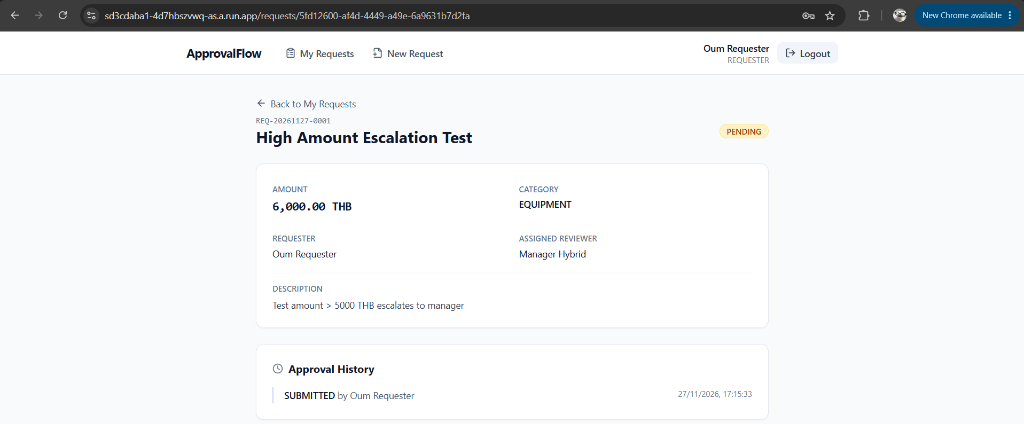
\includegraphics[width=0.82\textwidth]{evidence/screenshots/fig-changed-escalation.png}
\end{center}

\clearpage
% =====================================================================
% PAGE 6: Part D (Cont.) Screenshots, Teamwork, AI-Use & Limitations
% =====================================================================
\partheader{Part D (Cont.): Live Evidence, Team Contributions \& Governance}{Submission Package}

\textbf{Figure 2: Preserved Behavior Verification (\code{REQ-20261127-0002}) --- In-Hours Equipment Mapped to T Reviewer}
\begin{center}
  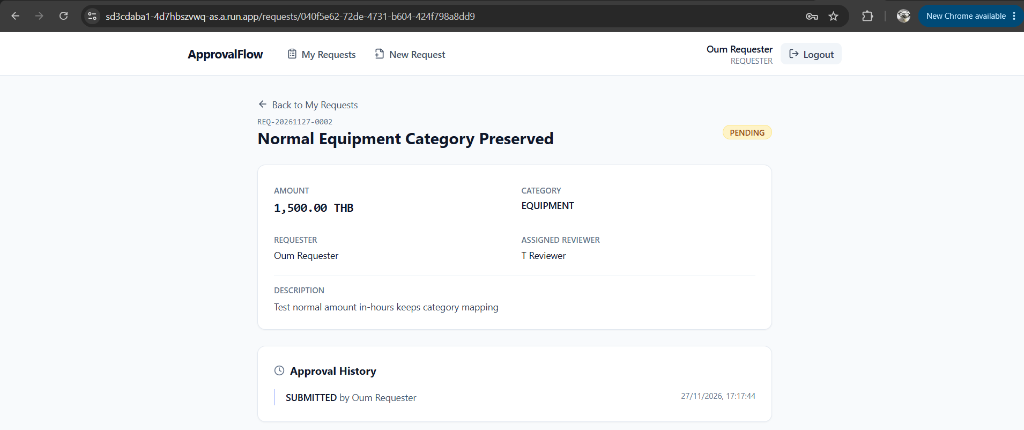
\includegraphics[width=0.82\textwidth]{evidence/screenshots/fig-preserved-normal.png}
\end{center}
\vspace{1pt}

\textbf{4. Balanced Team Contribution Table (50/50 Partnership):}
\begin{center}
\footnotesize
\begin{tabular}{@{}L{3.8cm}C{1.8cm}C{1.8cm}L{9.4cm}@{}}
\toprule
\textbf{Member Name} & \textbf{Student ID} & \textbf{GitHub} & \textbf{Core Roles \& Substantive Contributions in Lab 7} \\
\midrule
\textbf{Siriwan Yindeepot (Oum)} & 67070501075 & @ssiriwan & $\bullet$ Authored 6 automated boundary/security tests (RED commit \code{2b56a7b}).\newline $\bullet$ Implemented reviewer escalation logic (GREEN commit \code{fede788}).\newline $\bullet$ Configured Vitest fake timers and verified 43/43 regression suite.\newline $\bullet$ Reviewed and merged Release PR \#64 into \code{main}.\newline $\bullet$ Executed live Cloud Run verification tests (\code{REQ-20261127-0001} \& \code{0002}). \\
\midrule
\textbf{Thanaboon Tikaew (T)} & 67070501021 & @thhanabun & $\bullet$ Authored Part A change request, impact analysis, and contract v1.1 (PR \#61).\newline $\bullet$ Conducted substantive peer review on PR \#63 with CHANGES\_REQUESTED.\newline $\bullet$ Authored documentation refinements and process disclosures (commit \code{64d02c6}).\newline $\bullet$ Opened Release PR \#64 from \code{lab7-staging} to \code{main}.\newline $\bullet$ Verified Google Cloud Run deployment pipeline and health endpoints. \\
\bottomrule
\end{tabular}
\end{center}
\vspace{1pt}

\textbf{5. AI-Use Declaration \& Integrity Verification:}
\begin{itemize}[leftmargin=*,itemsep=1pt,topsep=1pt]
  \item \textbf{Tool Utilized:} Google Antigravity / Gemini code assistant.
  \item \textbf{Usage Scope:} (1) Drafting boilerplate Markdown contract templates and tables; (2) Formulating Vitest fake timer mock syntax (\code{{toFake: ['Date']}}) to prevent bcrypt timer interference; (3) Structuring LaTeX report formatting and table alignment.
  \item \textbf{Human Verification \& Safety:} Every line of code, automated test assertion, and command output was executed, audited, and verified locally by the human authors. Zero production credentials, Google Cloud service account keys, or database secrets were exposed to AI tools or committed to Git.
\end{itemize}

\textbf{6. Known Limitations \& Process Disclosures:}
\begin{enumerate}[leftmargin=*,itemsep=1pt,topsep=1pt]
  \item \textbf{Contract Review Sequence:} As honestly disclosed in \path{README.md} and PR \#63, formal teammate review of the revised contract was conducted during PR \#63 peer review rather than strictly prior to the implementation commit. No approval date or reviewer record was fabricated.
  \item \textbf{Instructor/TA Pre-Approval:} Course staff waived synchronous pre-approval for Lab 7; recorded honestly as \textbf{NOT AVAILABLE}.
  \item \textbf{Database Schema Evolution:} Zero schema changes were required for CR-04; historical requests created prior to Lab 7 retain original reviewer assignments and remain fully queryable.
\end{enumerate}

\end{document}
